\documentclass[12pt,twoside]{report}

%%%%%%%%%%%%%%%%%%%%%%%%%%%%%%%%%%%%%%%%%%%%%%%%%%%%%%%%%%%%%%%%%%%%%%%%%%%%%

% Definitions for the title page
% Edit these to provide the correct information
% e.g. \newcommand{\reportauthor}{Timothy Kimber}

\newcommand{\reporttitle}{Learning for SLAM in Dynamic Environments \\[1cm] Background Report}
\newcommand{\reportauthor}{Ciro Cursio}
\newcommand{\supervisor}{Stefan Leutenegger}
\newcommand{\degreetype}{Computing (Machine Learning)}

%%%%%%%%%%%%%%%%%%%%%%%%%%%%%%%%%%%%%%%%%%%%%%%%%%%%%%%%%%%%%%%%%%%%%%%%%%%%%

% load some definitions and default packages
%%%%%%%%%%%%%%%%%%%%%%%%%%%%%%%%%%%%%%%%%
% University Assignment Title Page 
% LaTeX Template
% Version 1.0 (27/12/12)
%
% This template has been downloaded from:
% http://www.LaTeXTemplates.com
%
% Original author:
% WikiBooks (http://en.wikibooks.org/wiki/LaTeX/Title_Creation)
%
% License:
% CC BY-NC-SA 3.0 (http://creativecommons.org/licenses/by-nc-sa/3.0/)
% 
%
%%%%%%%%%%%%%%%%%%%%%%%%%%%%%%%%%%%%%%%%%
%----------------------------------------------------------------------------------------
%	PACKAGES AND OTHER DOCUMENT CONFIGURATIONS
%----------------------------------------------------------------------------------------
\usepackage[a4paper,hmargin=2.8cm,vmargin=2.0cm,includeheadfoot]{geometry}
\usepackage{textpos}
%\usepackage{natbib} % for bibliography
\usepackage{tabularx,longtable,multirow,subfigure,caption}%hangcaption
\usepackage{fncylab} %formatting of labels
\usepackage{fancyhdr} % page layout
\usepackage{url} % URLs
\usepackage[english]{babel}
\usepackage{amsmath}
\usepackage{graphicx}
\usepackage{dsfont}
\usepackage{epstopdf} % automatically replace .eps with .pdf in graphics
\usepackage{backref} % needed for citations
\usepackage{array}
\usepackage{latexsym}
\usepackage[pdftex,pagebackref,hypertexnames=false,colorlinks]{hyperref} % provide links in pdf

\hypersetup{pdftitle={},
  pdfsubject={}, 
  pdfauthor={},
  pdfkeywords={}, 
  pdfstartview=FitH,
  pdfpagemode={UseOutlines},% None, FullScreen, UseOutlines
  bookmarksnumbered=true, bookmarksopen=true, colorlinks,
    citecolor=black,%
    filecolor=black,%
    linkcolor=black,%
    urlcolor=black}

\usepackage[all]{hypcap}


%\usepackage{color}
%\usepackage[tight,ugly]{units}
%\usepackage{float}
%\usepackage{tcolorbox}
%\usepackage[colorinlistoftodos]{todonotes}
% \usepackage{ntheorem}
% \theoremstyle{break}
% \newtheorem{lemma}{Lemma}
% \newtheorem{theorem}{Theorem}
% \newtheorem{remark}{Remark}
% \newtheorem{definition}{Definition}
% \newtheorem{proof}{Proof}


%%% Default fonts
\renewcommand*{\rmdefault}{bch}
\renewcommand*{\ttdefault}{cmtt}



%%% Default settings (page layout)
\setlength{\parindent}{0em}  % indentation of paragraph

\setlength{\headheight}{14.5pt}
\pagestyle{fancy}
\renewcommand{\chaptermark}[1]{\markboth{\chaptername\ \thechapter.\ #1}{}} 

\fancyfoot[ER,OL]{\sffamily\textbf{\thepage}}%Page no. in the left on odd pages and on right on even pages
\fancyfoot[OC,EC]{\sffamily }
\renewcommand{\headrulewidth}{0.1pt}
\renewcommand{\footrulewidth}{0.1pt}
\captionsetup{margin=10pt,font=small,labelfont=bf}


%--- chapter heading

\def\@makechapterhead#1{%
  \vspace*{10\p@}%
  {\parindent \z@ \raggedright \sffamily
    \interlinepenalty\@M
    \Huge\bfseries \thechapter \space\space #1\par\nobreak
    \vskip 30\p@
  }}

%---chapter heading for \chapter*  
\def\@makeschapterhead#1{%
  \vspace*{10\p@}%
  {\parindent \z@ \raggedright
    \sffamily
    \interlinepenalty\@M
    \Huge \bfseries  #1\par\nobreak
    \vskip 30\p@
  }}

\allowdisplaybreaks

% load some macros
% Here, you can define your own macros. Some examples are given below.

\newcommand{\R}[0]{\mathds{R}} % real numbers
\newcommand{\Z}[0]{\mathds{Z}} % integers
\newcommand{\N}[0]{\mathds{N}} % natural numbers
\newcommand{\C}[0]{\mathds{C}} % complex numbers
\renewcommand{\vec}[1]{{\boldsymbol{{#1}}}} % vector
\newcommand{\mat}[1]{{\boldsymbol{{#1}}}} % matrix


\date{June 2019}

\begin{document}

% load title page
% Last modification: 2015-08-17 (Marc Deisenroth)
\begin{titlepage}

\newcommand{\HRule}{\rule{\linewidth}{0.5mm}} % Defines a new command for the horizontal lines, change thickness here


%----------------------------------------------------------------------------------------
%	LOGO SECTION
%----------------------------------------------------------------------------------------


\includegraphics[width = 4cm]{./figures/imperial}\\[0.5cm] 

\center % Center remainder of the page

%----------------------------------------------------------------------------------------
%	HEADING SECTIONS
%----------------------------------------------------------------------------------------

\textsc{\Large Imperial College London}\\[0.5cm] 
\textsc{\large Department of Computing}\\[0.5cm] 

%----------------------------------------------------------------------------------------
%	TITLE SECTION
%----------------------------------------------------------------------------------------

\HRule \\[0.4cm]
{ \huge \bfseries \reporttitle}\\ % Title of your document
\HRule \\[2cm]
 
%----------------------------------------------------------------------------------------
%	AUTHOR SECTION
%----------------------------------------------------------------------------------------

\begin{minipage}{0.4\textwidth}
\begin{flushleft} \large
\emph{Author:}\\
\reportauthor % Your name
\end{flushleft}
\end{minipage}
~
\begin{minipage}{0.4\textwidth}
\begin{flushright} \large
\emph{Supervisor:} \\
\supervisor % Supervisor's Name
\end{flushright}
\end{minipage}\\[4cm]


%----------------------------------------------------------------------------------------
%	FOOTER & DATE SECTION
%----------------------------------------------------------------------------------------
\vfill % Fill the rest of the page with whitespace
Submitted in partial fulfillment of the requirements for the MSc degree in
\degreetype~of Imperial College London\\[0.5cm]

\makeatletter
\@date 
\makeatother


\end{titlepage}



% page numbering etc.
\pagenumbering{roman}
\clearpage{\pagestyle{empty}\cleardoublepage}
\setcounter{page}{1}
\pagestyle{fancy}


\cleardoublepage
%%%%%%%%%%%%%%%%%%%%%%%%%%%%%%%%%%%%
%\section*{Acknowledgments}
%Comment this out if not needed.

\clearpage{\pagestyle{empty}\cleardoublepage}

%%%%%%%%%%%%%%%%%%%%%%%%%%%%%%%%%%%%
%--- table of contents
\fancyhead[RE,LO]{\sffamily {Table of Contents}}
\tableofcontents 


\clearpage{\pagestyle{empty}\cleardoublepage}
\pagenumbering{arabic}
\setcounter{page}{1}
\fancyhead[LE,RO]{\slshape \rightmark}
\fancyhead[LO,RE]{\slshape \leftmark}

%%%%%%%%%%%%%%%%%%%%%%%%%%%%%%%%%%%%
\chapter{Introduction}

In recent times, computer vision applications have seen a dramatic rise in their popularity, from autonomous cars and robots to augmented reality systems. Their spatial awareness requirements are achieved by using Simultaneous Localisation and Mapping (SLAM), a strategy for jointly estimating a map of the environment and the position of the mapping agent in this environment: however, one of the biggest limitations of traditional SLAM algorithms is that the environment is assumed to be static, which limits the usefulness of this algorithm when the scene contains dynamic elements such as moving cars or people.
\\

In the last years we have started to see SLAM systems that take into account such dynamics using strategies that can be roughly divided in three classes:

\begin{itemize}
\item \textbf{Rejection of Dynamic Elements:} this approach focuses on actively ignoring dynamic elements and only mapping the static parts of the scene.
\item \textbf{Non-Rigid Object Reconstruction:} here the focus is on modelling only the dynamic parts of the scene, especially objects that deform in a non-rigid manner.
\item \textbf{Multi-Object Tracking:} this approach combines both static and dynamic information, thus being able to create a map of the static parts of the environment, and simultaneously reconstruct and map moving objects that move rigidly.
\end{itemize}

The approaches that reject dynamic elements tend to have a high tracking accuracy of the camera pose \cite{staticfusion}, while approaches that reconstruct non-rigid objects can deal with extreme transformations \cite{dynamicfusion, fusion4d}. However, the strategy that has the largest potential and room for expansion is the one based on multi-object tracking \cite{cofusion, maskfusion, midfusion}: this approach tracks an arbitrary number of moving objects, thus allowing a greater degree of interaction between the agent and the environment (think of a robot manipulating objects in a room, or a virtual reality system that reacts when an object in the scene is moved).
\\

At the core of such systems is a segmentation strategy that can distinguish between the camera pixels belonging to each moving object and the pixels belonging to the background. While the first dynamic SLAM systems focused on separating the static parts and moving parts of the scene based on motion cues \cite{cofusion}, in the last two years the focus shifted to semantic SLAM, where a deep learning-based segmentation system is used to identify each object and detect the region it occupies in the camera image. This presents a great advantage in the level of awareness that the agent gains (shifting from simply mapping the environment to understanding it), however it also introduces a significant speed limitation, since almost all segmentation networks are only optimised for accuracy and not speed: as a result, the state of the art systems for semantic instance segmentation currently integrated in SLAM systems operate at a maximum of 5 Hz on expensive high-end GPUs.
\\

This bottleneck is currently limiting dynamic SLAM systems in two aspects: first, it reduces their tracking capabilities in scenarios where the scene contain fast-moving elements, or when the agent itself performs rapid movements; second, it requires significant computational power, which in turn requires powerful hardware that is both expensive and cumbersome, especially on smaller robots and virtual reality headsets. This is the main problem that the present thesis aims to address: how can we improve the operating frequency of instance segmentation in the context of dynamic SLAM without a degradation in performance?
\\
\\

\section{Aims and Objectives}

The two main targets of this thesis are thus outlined below:

\begin{itemize}
\item \textbf{Development of a fast segmentation architecture:} following a literature review (included in this report) of the current methods for instance segmentation, the highest performing architectures in both accuracy and speed will be experimented with, and the insight gained will be used to build an architecture that reaches the target operating frequency of 30 Hz with the smallest possible degradation in segmentation accuracy compared to the state of the art.
\item \textbf{Integration with an existing dynamic SLAM system:} in order to measure the real-world effectiveness of such a segmentation system, it will need to be integrated in a current dynamic SLAM system that employs moving object tracking, possibly one where the segmentation system is the computational bottleneck. After integration, the change in operating frequency, camera tracking and object reconstruction accuracy will be measured.
\end{itemize}

In addition, we define some additional targets that are not critical to the completion of the thesis, but present additional areas that could be interesting to explore:

\begin{itemize}
\item \textbf{Integration of depth information:} the most recent SLAM systems make use of RGBD cameras, which provide depth information together with RGB colour. However, the state of the art semantic segmentation methods only make use of RGB images, thus making it desirable for the SLAM system to further refine the segmentation masks using the scene depth in a subsequent and separate step. An alternative could be to integrate the depth refinement in the segmentation network, which could result in a speed-up compared to having two separate steps.
\item \textbf{Amodal instance semantic segmentation:} defined as the segmentation of objects \textit{including the parts that are occluded by other objects}, amodal segmentation could improve object tracking in dynamic SLAM, as the object pose would be easier to estimate in difficult situations with many occlusions. However, amodal segmentation is an extremely recent research field, and thus the level of performance of the current methods is not as high as in the modal counterpart. This presents both a greater opportunity for original work, and a higher level of difficulty in creating a well-performing system.
\end{itemize}


%%%%%%%%%%%%%%%%%%%%%%%%%%%%%%%%%%%%
\chapter{Background}

\section{Semantic Segmentation}

Semantic segmentation, also defined as dense classification, is the labelling of each individual pixel in an image as belonging to a particular class of objects. The key difference between segmentation and a more baseline approach such as image classification or object detection is that the output of a semantic segmentation system is an image with the same resolution as the input image. For completeness, we should say that deep learning is not the only method for performing semantic segmentation: Conditional Random Fields (CRF) were extensively used before deep learning rose in popularity, however the performance achieved by such systems is much lower than recent deep learning-based methods, so in this project we will only focus on deep learning-based methods. 
\\

The need for a pixel-wise output is directly reflected on the general architecture of segmentation systems as opposed to more traditional convolutional neural networks (CNN) used for image classification.

Standard CNNs used for image classification are usually built as an interleaved sequence of convolutional layers and downsampling layers, or, in alternative, a sequence of convolutional layers with a stride larger than 1. This causes them to have smaller and smaller feature maps as layers get deeper, the intuition behind it being that the deeper layers already build on the outputs of the previous layers, learning features based on previous features, so they need to retain only the information that is most useful for classifying the image.

On the other hand, semantic segmentation networks are frequently based on an encoder-decoder architecture: the encoder part performs downsampling and feature extraction in a similar fashion to traditional CNNs, in order to build a latent representation of the image that only contains the most useful features for segmentation; the decoder part takes this latent representation and performs upsampling by using either an interleaved sequence of convolutional layers and interpolation (e.g. nearest neighbour or bilinear), or a sequence of fractionally-strided convolutions, the final output being a rescaled image that contains a class output for each pixel. The difference in general architecture is illustrated in the image below: 
\\

\begin{figure}[ht]%[tb]
\centering
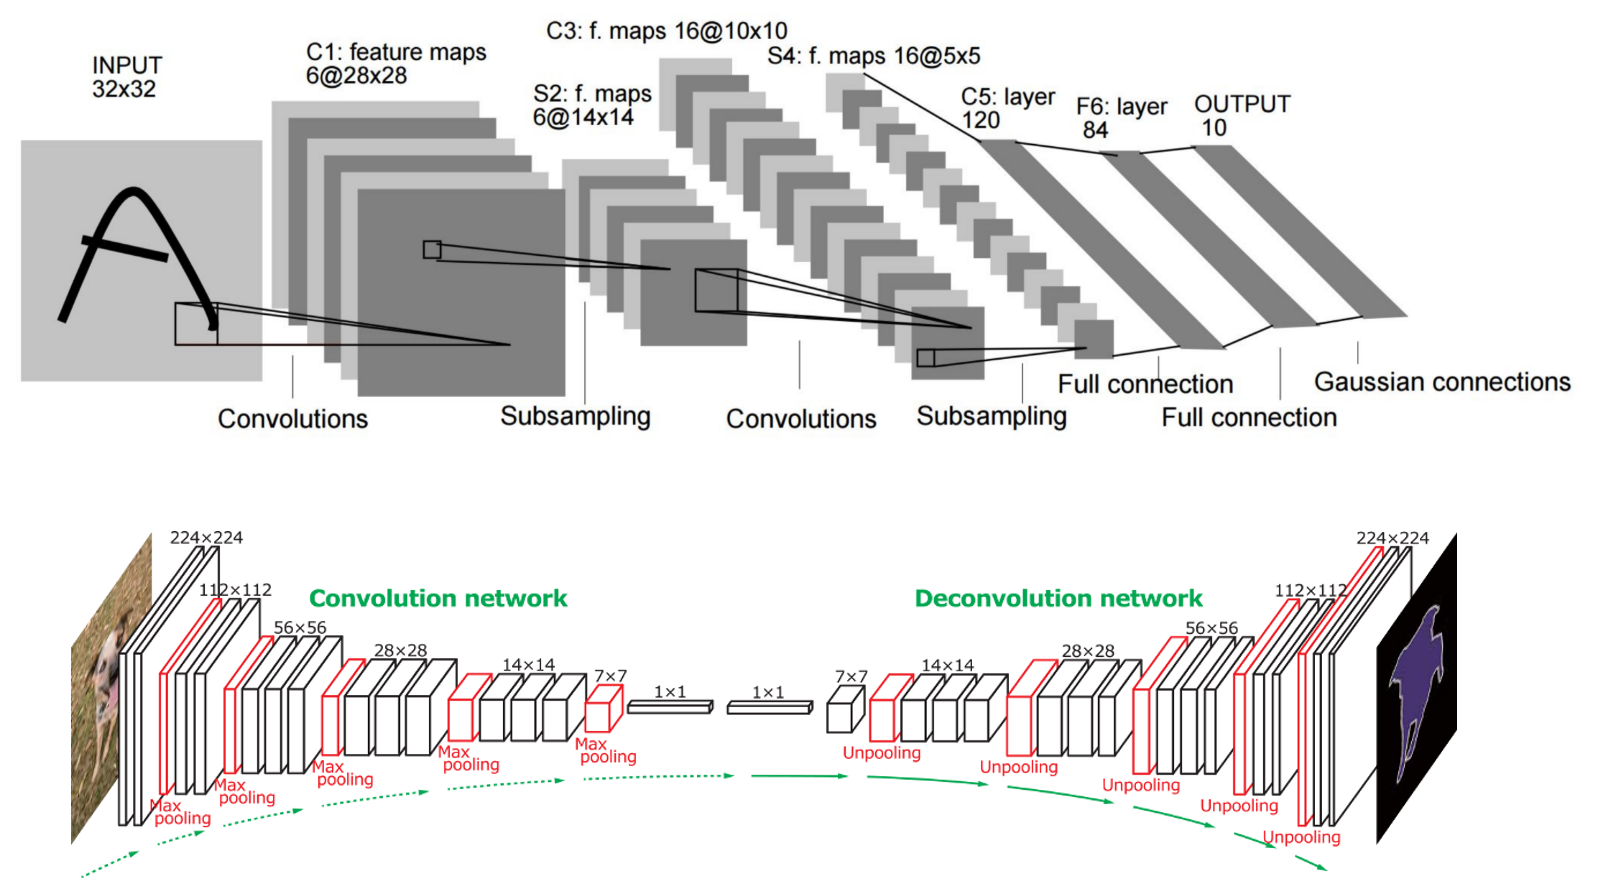
\includegraphics[width = 1\hsize]{./figures/cnn-ed}
\caption{Comparison of a standard CNN used for classification (above) \cite{cnn} and an encoder-decoder used for segmentation (below) \cite{encdec}. It can be seen that the encoder-decoder is formed by stacking a CNN and an inverted CNN. Note: if the CNN does not contain fully connected layers like the figure above, then it is called Fully Convolutional Network (FCN).}
\label{fig:cnn-ed}
\end{figure}

Many further improvements were added to the standard CNN formulation in recent years. One of the most effective modifications was the addition of skip connections, popularised in the ResNet architecture \cite{resnet}. These are direct connections between non-adjacent layers originally intended to reduce the effect of the vanishing gradient problem: the result is a building block with two parallel datapaths, one with a short number of convolutional layers (usually two or three) and the other being the skip connection. This trick allowed to build much deeper neural networks than it was previously possible, making networks with hundreds or even thousands of layers possible; furthermore, in the context of semantic segmentation, these connections allow information from different resolutions to be directly accessible in deeper layers, thus making the system able to take advantage of multi-resolution information at each layer. An analogous strategy is employed in the Inception v4 network \cite{inceptionv4}, where different convolutional blocks are executed in parallel and then their outputs are concatenated together to be fed to the next Inception block. Such concepts are not dissimilar from the spatial pyramid pooling introduced in \cite{spp}, where the last convolutional layer of the CNN is subjected to a multi-resolution pooling and then the outputs of the pooling operations are concatenated together to yield a fixed-length vector containing information at multiple resolutions. These three architectures are illustrated in figure \ref{fig:skip-connections} to show their similarity.
\\

\begin{figure}[ht]%[tb]
\centering
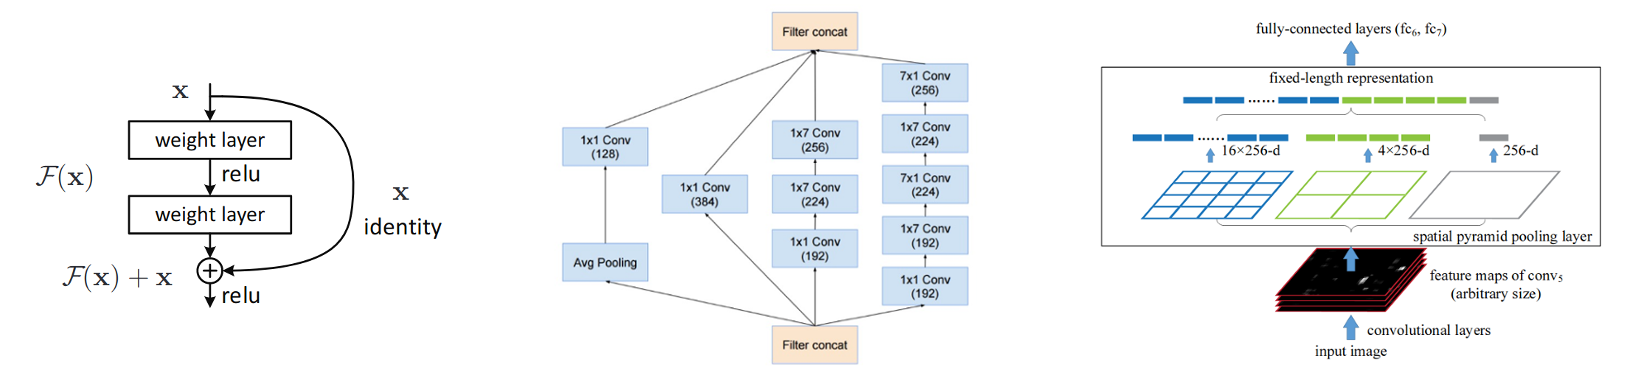
\includegraphics[width = 1.05\hsize]{./figures/skip-connections}
\caption{ResNet block (left) \cite{resnet}, Inception v4 B block (centre) \cite{inceptionv4} and CNN using spatial pyramid pooling (right) \cite{spp}.}
\label{fig:skip-connections}
\end{figure}

All the most recent and accurate semantic segmentation systems rely on one or more of the concepts introduced by these classification networks: an example is \cite{revisitingresnets}, where a thorough analysis of the effects of skip connections in ResNets is carried out, and the results are used to determine the optimal size of a ResNet building block (which was found to be a sequence of two convolutional layers with a kernel size of 3x3 each): a ResNet-based architecture is then created and trained for semantic segmentation, achieving state of the art results on a number of segmentation datasets such as Cityscapes, PASCAL VOC and PASCAL Context. An even more recent example is Deeplab v3+ \cite{deeplabv3+}, based on an encoder-decoder architecture where the last layer of the encoder is a spatial pyramid pooling layer. The paper also makes extensive use of atrous convolution, where the filter kernel can be dilated with a learnt parameter in order to cover a larger area without increasing computational cost.


\section{Instance Segmentation}

We have briefly examined semantic segmentation and the defining traits of the contemporary deep learning-based segmentators. Instance semantic segmentation, or instance segmentation in short, is an extension of semantic segmentation that is more relevant to SLAM for a key reason: where semantic segmentation only labels pixels belonging to a certain class, instance segmentation also distinguishes between different objects belonging to the same class, so each pixel will not only be labeled with a class, but also with an instance number. This makes instance segmentation much more useful for SLAM, as it allows to distinguish and track different objects even if they belong to the same class, but it also constitutes a considerably more difficult problem than semantic segmentation, as the level of similarity between instances of a certain object in an image can be extremely variable. A task that is closely related to instance segmentation is object detection, where instances of each class are located in the image and outlined with a bounding box without any kind of pixel-by-pixel labelling occurring. We will spend some time outlining object detection methods, because all instance segmentation algorithms are derived from a corresponding object detection algorithm.
\\

Early object detection approaches were mainly focused on performing standard classification on a window sliding over the image in order to localise the occurrences of an instance, however this approach proved to be extremely computationally expensive: since the instances of a class can be very varied in size and shape, a huge number of different windows need to be examined and the classification network needs to be run on each one of them.
\\

To solve this problem, object detection algorithms evolved into a two-stage approach: first, a number of regions in the image are proposed; then, a CNN is used to classify each proposed region. This approach was pioneered by Region-CNN (RCNN) \cite{rcnn}, which employs selective search to generate around 2000 proposals: these proposed regions are then classified by the CNN which produces a latent vector; this vector is then fed to a support vector machine for classification, and a bounding box regressor which yields a refined bounding box for the object in the region. This approach still had a number of limitations, the largest of which was that both training and inference times were extremely long, as the CNN had to be run 2000 times for each image it was presented with. However, RCNN formed the basis for a huge number of object detection and instance segmentation algorithms.
\\

Direct followers of RCNN are Fast-RCNN \cite{fastrcnn} and Faster-RCNN \cite{fasterrcnn}. Fast-RCNN makes use of an FCN which takes the original image together with region proposals from the selective search, and outputs a feature map of the image. Then, for each region proposal, the feature map is fed to a Region of Interest (RoI)-pooling layer that outputs a fixed length feature vector, which is then passed onto a fully-connected network for both classification and bounding box regression. The advantage over RCNN is that this system is end-to-end trainable, while RCNN required separate training phases for each of its components, and this allowed it to achieve a higher bounding box accuracy.

Faster-RCNN eliminates the selective search, substituting it with two FCNs: a backbone network, which takes the input image and outputs a feature map, and a Region Proposal Network (RPN) which is slid over the feature map and outputs a set of object proposals. This architecture can be seen in the figure below:

\begin{figure}[ht]%[tb]
\centering
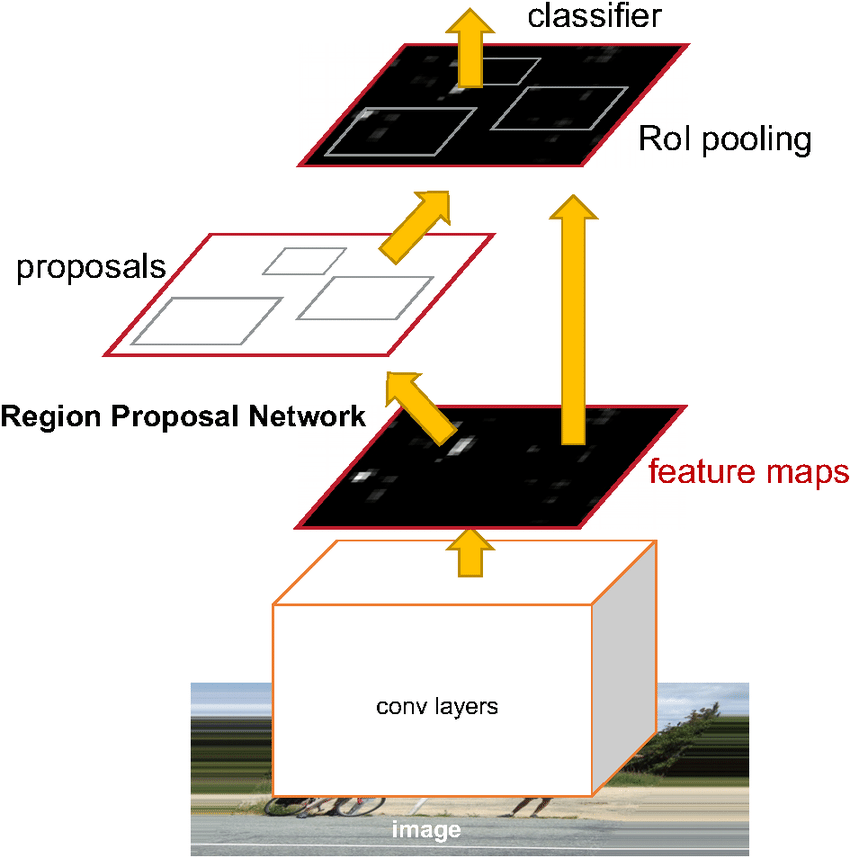
\includegraphics[width = 0.35\hsize]{./figures/faster-rcnn}
\caption{Faster-RCNN pipeline \cite{fasterrcnn}. We can see the main blocks, especially the backbone network (bottom), the RPN (middle) and the classification + bounding box regression (top).}
\label{fig:faster-rcnn}
\end{figure}

The main difference with Fast-RCNN is that the backbone + RPN network is trained to output high-quality object proposals, as opposed to selective search with relies on hand-crafted features: the consequence is that Faster-RCNN can afford to produce a lower number of proposals (300 instead of 2000), resulting in a significant speedup over previous methods. Faster-RCNN is the basis for an entire class of instance segmentation architectures, as we will see in the next section.
\\
\\

\textbf{Proposal-Based Segmentation}
\\

These segmentation systems follow the region proposal method pioneered by RCNN and expanded upon by Fast-RCNN and Faster-RCNN. Its main exponent is Mask-RCNN \cite{maskrcnn}, a very successful instance segmentation algorithm based on the Faster-RCNN architecture. Published in 2017, this algorithm quickly became the state of the art for instance segmentation, still being very competitive as of today in terms of both accuracy and computational cost, so much so that all the most recent dynamic SLAM systems that make use of semantic segmentation use Mask-RCNN. It should still be remarked that the maximum operating frequency of Mask-RCNN is around 5 Hz, thus not quite affording real-time operation.
\\

The architecture of Mask-RCNN is outlined here:

\begin{figure}[ht]%[tb]
\centering
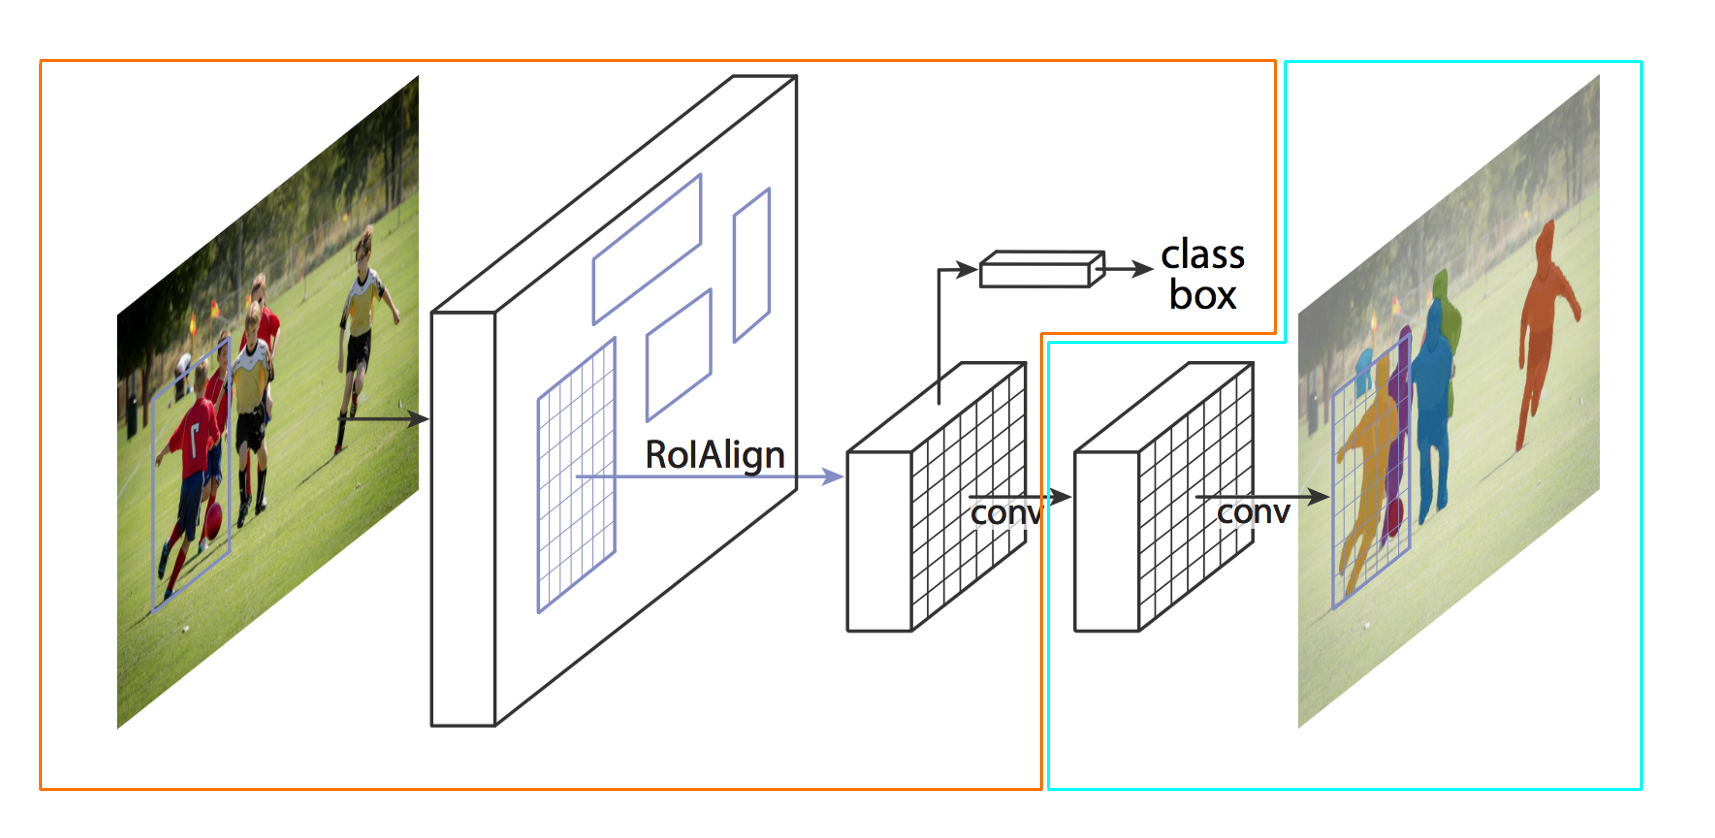
\includegraphics[width = 1\hsize]{./figures/maskrcnn}
\caption{Mask-RCNN pipeline \cite{maskrcnn}. The part in the orange contour is equivalent to Faster-RCNN except for the RoI-Align layer, while the part in the cyan contour is the mask branch.}
\label{fig:maskrcnn}
\end{figure}

We can see that it is very similar to Faster-RCNN, with the main difference being a "third branch" in addition to the classification branch and the bounding box regression branch. This third branch is composed of a small FCN that takes the feature map of the backbone network and outputs a simple binary mask that locates the object in the map. A key difference between Mask-RCNN and its object detection counterpart is how it handles RoIs: simply pooling them would result in inaccurate localisation, as the spatial information is quantised and thus fine details lost. Mask-RCNN substitutes the RoI-pool layer of Fast-RCNN with an RoI-align layer, which does not quantise the position of the pixels to be pooled, but performs bilinear interpolation to find the pixel colours and only then it performs pooling. This small difference leads to a huge improvement in segmentation accuracy as noted in the ablation study conducted by the authors, and it seems to be the key feature which allowed Mask-RCNN to reach such high accuracy compared to the competition. Another key insight is the decoupling of mask and class predictions: the mask branch of Mask-RCNN has no class information, while traditional FCNs perform classification on each pixel, putting all classes in competition with each other, which was noted by the authors to yield worse results in instance segmentation tasks. Further, the authors experimented with different backbone networks among ResNets, ResNeXts and Feature Pyramid Networks (FPNs), a recent encoder-decoder architecture that includes symmetric skip connections between the feature maps of the encoder and the feature maps of the decoder that have the same resolution: predictions are then output by all the layers of the decoder simultaneously, so that region proposals at very different scales can be found. This architecture proved to be the best performer as a Mask-RCNN backbone.
\\

A successor to Mask-RCNN is the Path Aggregation Network (PANet) \cite{panet}, currently the state of the art on the COCO Instance Segmentation Challenge and the Cityscapes dataset. This architecture uses a modified FPN backbone with a bottom-up path augmentation, which consists in an additional encoder-like structure at the end of the FPN, with skip-connections at each layer going to each corresponding layer in the decoder of the FPN. These shortcuts result in a better combination of features at multiple resolutions. Furthermore, for each region proposed by this augmented FPN, its correspondents in all layers in the path augmentation are found and versions of the same region at multiple resolutions are obtained; features from these regions are then pooled and passed to the classification, bounding box and mask branches.

While this paper achieves an impressive level of accuracy, it should be noted that it also introduces additional latency compared to Mask-RCNN, thus making it even less convenient for SLAM applications than Mask-RCNN.
\\

Despite their popularity, such systems based on region proposal are affected by two limitations, the first one being that they have an upper bound on the number of object instances they can process in a single image (limited by the number of proposals provided by the RPN network), and the second being that they will have to execute classification and masking on each proposal, which is computationally expensive. It should also be mentioned that the convolutional operators used in all these systems might not be a natural fit for instance segmentation tasks, because convolution is translation equivariant and thus it cannot distinguish between object instances that look the same but are in different locations of the image. \cite{semiconvolutional} introduces a semi-convolutional operator, which is the sum of convolution and the pixel location in the image, so that position information is embedded in the operator, and a modified version of Mask-RCNN with this operator outperforms the original algorithm, thus suggesting that these operators might be better suited to instance segmentation than simple convolution.
\\

In the next section we will explore instance segmentation approaches based on a completely different principle: instead of proposing a high number of regions and then performing classification and segmentation on them, they implement a single shot strategy where all the object instances are segmented in only one pass over the input image, which has the potential of being much faster than proposal-based methods.
\\
\\

\textbf{Single Shot Segmentation}
\\

As in the case of proposal-based segmentation, single shot instance segmentation has its roots in single shot object detection, whose main exponents are You Only Look Once (YOLO) and Single Shot Detector (SSD).
\\

YOLO \cite{yolo} treats object detection as a regression problem, dividing the input image in a grid of 7x7 squares and then simultaneously performing classification and regression of two bounding boxes for each square. This simple pipeline has a huge speed advantage over proposal-based methods: in fact, YOLO can perform object detection at 45 Hz, which is an enormous improvement over the 7 Hz achieved by Faster-RCNN with a VGG-16 backbone, while detection accuracy is on par, if slightly lower, than Faster-RCNN.

YOLO had a number of evolutions in the last years such as YOLO9000 \cite{yolo9000}, which applies a large number of improvements to YOLO such as dramatically increasing the number of predicted bounding boxes (the original YOLO proposed 98 boxes, YOLO9000 can propose more than a thousand) and using a much faster architecture (called DarkNet-19 by the authors): the result is an operating frequency of 67 Hz and an accuracy that outperforms Faster-RCNN; the latest development is represented by YOLOv3 \cite{yolov3}, which is based on DarkNet-53, an architecture which contains skip connections. YOLOv3 operates at a similar frequency as YOLO9000 but it achieves slightly higher accuracy. 
\\

SSD \cite{ssd} builds on the original YOLO by dividing the image in an 8x8 grid, each square proposing 4 boxes with different sizes and aspect ratios. Then, for each box, an offset is predicted to refine its size and location; further, unlike YOLO, SSD combines feature maps from multiple resolutions to predict boxes at vastly different scales. This allows it to achieve a higher accuracy than Faster-RCNN while being faster than both Faster-RCNN and YOLO (60 Hz), also allowing it to produce a vastly higher number of boxes (8732).
\\

In the context of instance segmentation single shot systems are extremely recent, so much so that the papers examined here were published in this current year. The first one is You Only Look At CoefficienTs (YOLACT) \cite{yolact}. YOLACT breaks the problem into two parallel tasks. The first one consists in generating a set of prototype masks with the same size as the input image: these prototypes don't directly contain any object masks, instead they learn spatial information over the whole image such as contours or space partitioning. The second task is to predict a coefficient for each prototype mask and four instances for each class: these two tasks are combined together by performing a linear combination of the prototype masks using the predicted coefficients, and the result is subjected to a sigmoid activation to yield a binary mask for each instance.

Thanks to this lightweight formulation for instance segmentation, YOLACT is the first instance segmentator that can run in real-time, going above a 30 Hz operating frequency. However its accuracy, while not terrible, is not on the same level as Mask-RCNN.
\\

A slightly older approach based on a different concept is constituted by the Deep Watershed Transform (DWT) \cite{deepwatershed}. In this paper, the authors build a deep-learning version of the watershed transform, a very popular segmentation filter which represent the image as a topographical surface with peaks and troughs: from a conceptual point of view, the filter is equivalent to water being dropped on this topographical surface and collecting in the troughs: the surface can then be cut at water level to create the segmentation (which often results in oversegmentation of the image). The contribution of this paper is that the DWT learns a topographical representation of the image so that the peaks are in correspondence of the boundaries between instances. This is achieved by chaining two neural networks, a Direction Network (DN) and a Watershed Transform Network (WTN): the DN outputs a 2D field of unit vectors which point away from the nearest instance boundary. This has the purpose of simplifying training by creating a robust representation for the instance boundaries, since the difference in the direction of these vectors is very big in proximity to instance boundaries (the vectors on one side will be pointing almost in the opposite direction to the vectors on the other side). This 2D field, which has the same resolution as the input image, is then passed onto the WTN, which outputs an energy map that is zero at pixels close to the instance boundaries and increases in value as the pixels get farther from the boundaries. The architecture of these two networks is shown below:
\\

\begin{figure}[ht]%[tb]
\centering
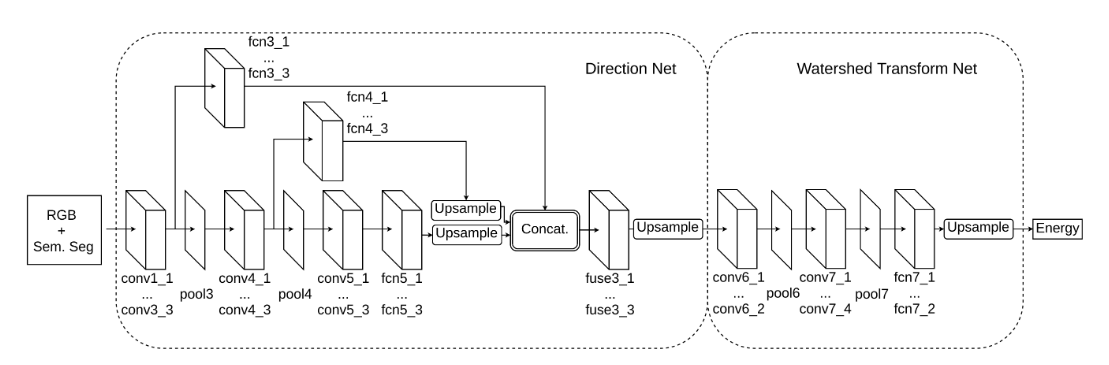
\includegraphics[width = 0.74\hsize]{./figures/dwt}
\caption{Deep watershed transform pipeline \cite{deepwatershed}. Direction network is on the left, watershed transform network on the right.}
\label{fig:dwt}
\end{figure}

Comparing the performance of the DWT with the other segmentation methods is not an easy task, as this algorithm was created with autonomous cars in mind, so the datasets on which it was evaluated and the accuracy metric used are different. Furthermore, this system requires an image which has already been segmented into its main semantic components: this puts a limitation on its usefulness, but also creates an opportunity for expansion to an all-in-one instance semantic segmentation based on the watershed transform. Finally, the authors don't mention any timing information, but we can infer from the very simple architecture of the two networks that the overhead introduced over a semantic segmentation system won't be high compared to the systems that were examined in the previous paragraphs.


%%%%%%%%%%%%%%%%%%%%%%%%%%%%%%%%%%%%
\chapter{Project Setup}

\section{Plan}

The logistics of the project are outlined in the Gantt chart in figure \ref{fig:gantt}.
\\

\begin{figure}[hbtp]%[tb]
\centering
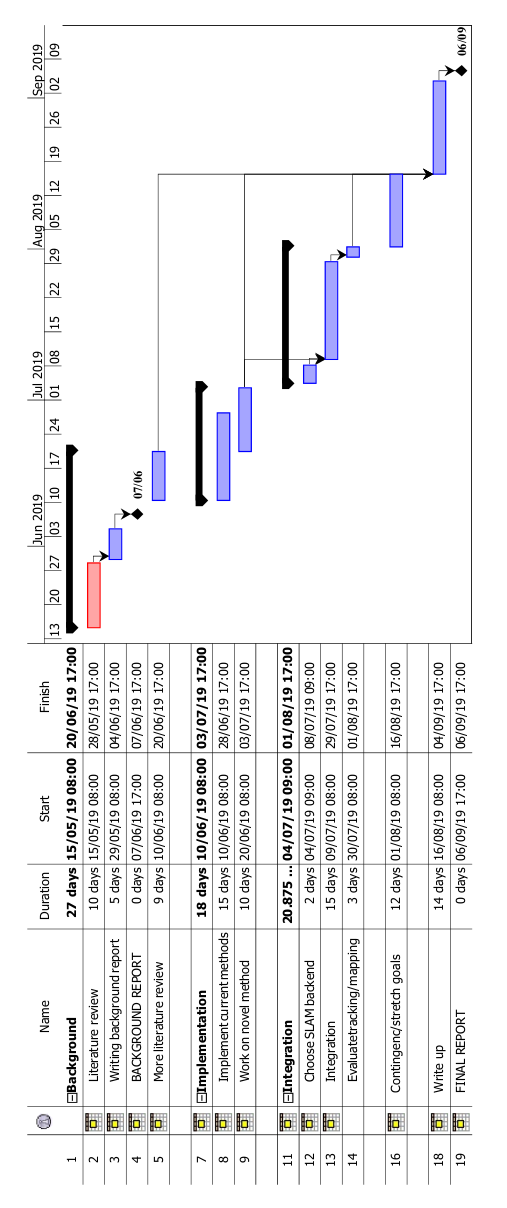
\includegraphics[width = 0.65\hsize]{./figures/gantt}
\caption{Gantt chart of thesis.}
\label{fig:gantt}
\end{figure}

Following from the aims and objectives of the thesis, the project has been divided into three stages.
\\

The first stage, mainly consisting in background research and a literature review, started at the beginning of the semester, and culminates with the present report; however, literature review may continue even after this report is completed, as new methods may be discovered or published in the meantime.
\\

In the second stage, the implementation of a novel instance segmentation system will be executed in a two-step fashion: first, the architectures of the highest performing segmentation systems will be reproduced on a local machine, their performance compared and their components analysed to better understand how they contribute to produce accurate instance segmentations; then, a novel instance segmentation will be created. It should be noted that this two-step stage is likely to be executed iteratively, jumping back and forth between step one and step two. This will facilitate the creation of a fall-back option in case of delays.
\\

The third stage of the project will consist in integrating the novel segmentation system in an existing SLAM pipeline to demonstrate its usability in a real-world scenario. We will choose a recent SLAM system that already employs an instance segmentation method for tracking moving objects: this will make it both easier to integrate the novel segmentation method, and to measure the improvements in timings, camera tracking and object reconstruction accuracy.
\\

Finally, 2-3 weeks in August have been left out for exploring the stretch goals of the project, or in alternative as contingency time for the main goals in case unforeseeen circumstances delay the completion of the thesis.


\section{Work Tools}

\textbf{Hardware}
\\

All proposed models will be trained on a local machine with the following specifications:

\begin{itemize}
\item CPU: AMD Ryzen 7 2700X
\item System memory: 32 GB
\item GPU: 2 x NVidia RTX 2080 TI, 11 GB of memory each
\end{itemize}

Such a machine should be powerful enough to train any segmentation network. Furthermore, the RTX series of GPUs are optimised for half-float (16 bit) computation, which would allow to train even larger models with larger batch sizes.
\\
\\

\textbf{Software}
\\

For the implementation stage of the project, the required software tools will be Python and a deep learning framework. Pytorch has been chosen because of the quicker development cycle it allows compared to Tensorflow, which is crucial in such a project where fast experimentation is key. Further, models can be easily ported to C++, which will be needed in the second stage of the project when the segmentation system will be integrated in a SLAM system, which will be written in C++.

%%%%%%%%%%%%%%%%%%%%%%%%%%%%%%%%%%%%
\chapter{Conclusion}

In this report we have specified the aims and objectives of the thesis, separating them into core objectives and optional goals: this will make it less likely to waste time exploring research areas that are not relevant to the main objectives.
\\

The results of the literature review were also outlined: we gave an exposition of the two main approaches to instance semantic segmentation and we described the most successful exponent for each approach. Following from this review, we gain the insight that proposal-based segmentators tend to achieve a higher accuracy at slower speeds, while single shot segmentators tend to achieve a very fast operating frequency, at a lower accuracy. Thus it is likely that a novel segmentation architecture for real-time operation will have a single shot pipeline at its core, and two directions for this project would be to make this single shot system more accurate so that it can compete with the state of the art in proposal-based segmentation, or to make the system even faster so that it can run at a high framerate even on less powerful hardware, without significant loss of accuracy.
\\

Lastly, the project plan was laid out as a Gantt chart and the main blocks were outlined: it was chosen to keep a high-level separation of tasks because the project is still at an early stage and thus modifications are likely to happen.


%%%%%%%%%%%%%%%%%%%%%%%%%%%%%%%%%%%%
\clearpage
\addcontentsline{toc}{chapter}{Bibliography}
%% bibliography
\bibliographystyle{ieeetr}
\bibliography{progress-refs}


\end{document}
